\documentclass[12pt,a4paper]{article}
\usepackage{amsmath,amssymb,mathrsfs,tikz,times,pifont}
\usepackage{enumitem}
\usepackage{multicol}
\usepackage{lmodern}
\usepackage{diagbox}
\usepackage{fancybox} % pour encadrer les résultats
\newcommand\circitem[1]{%
\tikz[baseline=(char.base)]{
\node[circle,draw=gray, fill=red!55,
minimum size=1.2em,inner sep=0] (char) {#1};}}
\newcommand\boxitem[1]{%
\tikz[baseline=(char.base)]{
\node[fill=cyan,
minimum size=1.2em,inner sep=0] (char) {#1};}}
\setlist[enumerate,1]{label=\protect\circitem{\arabic*}}
\setlist[enumerate,2]{label=\protect\boxitem{\alph*}}
\everymath{\displaystyle}
\usepackage[left=1cm,right=1cm,top=1cm,bottom=1.7cm]{geometry}
\usepackage[colorlinks=true, linkcolor=blue, urlcolor=blue, citecolor=blue]{hyperref}
\usepackage{array,multirow}
\usepackage[most]{tcolorbox}
\usepackage{varwidth}
\usepackage{float}
\tcbuselibrary{skins,hooks}
\usetikzlibrary{patterns}

\newtcolorbox{exa}[2][]{enhanced,breakable,before skip=2mm,after skip=5mm,
colback=yellow!20!white,colframe=black!20!blue,boxrule=0.5mm,
attach boxed title to top left ={xshift=0.6cm,yshift*=1mm-\tcboxedtitleheight},
fonttitle=\bfseries,
title={#2},#1,
boxed title style={frame code={
\path[fill=tcbcolback!30!black]
([yshift=-1mm,xshift=-1mm]frame.north west)
arc[start angle=0,end angle=180,radius=1mm]
([yshift=-1mm,xshift=1mm]frame.north east)
arc[start angle=180,end angle=0,radius=1mm];
\path[left color=tcbcolback!60!black,right color = tcbcolback!60!black,
middle color = tcbcolback!80!black]
([xshift=-2mm]frame.north west) -- ([xshift=2mm]frame.north east)
[rounded corners=1mm]-- ([xshift=1mm,yshift=-1mm]frame.north east)
-- (frame.south east) -- (frame.south west)
-- ([xshift=-1mm,yshift=-1mm]frame.north west)
[sharp corners]-- cycle;
},interior engine=empty,
},interior style={top color=yellow!5}}

\usepackage{fancyhdr}
\usepackage{eso-pic}
\usepackage{tkz-tab}
\usepackage{float} %pour utiliser l'option [H] qui force l'image à apparaître exactement à l'endroit où elle est placée dans le code.
\AddToShipoutPicture{
    \AtTextCenter{%
        \makebox[0pt]{\rotatebox{80}{\textcolor[gray]{0.7}{\fontsize{5cm}{5cm}\selectfont PGB}}}
    }
}
\usepackage{lastpage}
\fancyhf{}
\pagestyle{fancy}
\renewcommand{\footrulewidth}{1pt}
\renewcommand{\headrulewidth}{0pt}
\renewcommand{\footruleskip}{10pt}
\fancyfoot[R]{\color{blue}\ding{45}\ \textbf{2025}}
\fancyfoot[L]{\color{blue}\ding{45}\ \textbf{Prof : M. BA}}
\cfoot{\bf \thepage / \pageref{LastPage}}

\newcommand{\exo}[1]{%
        \textbf{\underline{Exercice #1}}
}

\begin{document}
\renewcommand{\arraystretch}{1.5}
\renewcommand{\arrayrulewidth}{1.2pt}
\begin{tikzpicture}[overlay,remember picture]
    \node[draw=blue,line width=1.2pt,fill=purple,text=blue,inner sep=3mm,rounded corners,pattern=dots]at ([yshift=-2.5cm]current page.north) {\begingroup\setlength{\fboxsep}{0pt}\colorbox{white}{\begin{tabular}{|*1{>{\centering \arraybackslash}p{0.28\textwidth}} |*2{>{\centering \arraybackslash}p{0.2\textwidth}|} *1{>{\centering \arraybackslash}p{0.19\textwidth}|} }
                \hline
                \multicolumn{3}{|c|}{$\diamond$$\diamond$$\diamond$\ \textbf{Lycée de Dindéfélo}\ $\diamond$$\diamond$$\diamond$ } & \textbf{A.S. : 2024/2025} \\ \hline
                \textbf{Matière : Mathématiques} & \textbf{Niveau : T S2} & \textbf{Date : 29/05/2025} & \textbf{} \\ \hline
                \multicolumn{4}{|c|}{\parbox[c]{10cm}{\begin{center}
                  \textbf{{\Large\sffamily Correction TD : Statistiques}}
                \end{center}}} \\ \hline
            \end{tabular}}\endgroup};
\end{tikzpicture}
\vspace{3cm}
\noindent
\section*{\underline{Exercice 1}( points)(BAC 2005)}
\begin{enumerate}
    \item Calcul du coefficient de corrélation linéaire

\[
r = \frac{\text{cov}(x, y)}{\sqrt{V(x)} \sqrt{V(y)}}
\]

\[
\bar{x} = \frac{1}{8} \sum_{i=1}^{8} x_i = \frac{60 + 80 + 100 + 120 + 140 + 160 + 180 + 200}{8} = \frac{1040}{8} = 130
\]

\[
\bar{y} = \frac{1}{8} \sum_{i=1}^{8} y_i = \frac{952 + 805 + 630 + 522 + 510 + 324 + 205 + 84}{8} = \frac{4032}{8} = 504
\]

\[
V(x) = \frac{1}{8} \sum_{i=1}^{8} x_i^2 - \bar{x}^2 = \frac{152000}{8} - (130)^2 = 2100
\]

\[
V(y) = \frac{1}{8} \sum_{i=1}^{8} y_i^2 - \bar{y}^2 = \frac{2637870}{8} - (504)^2 = 75717{,}75
\]

\[
\text{cov}(x, y) = \frac{1}{8} \sum_{i=1}^{8} x_i y_i - \bar{x} \bar{y} = \frac{424100}{8} - 130 \times 504 = -12507{,}5
\]

\[
r = \frac{-12507{,}5}{\sqrt{2100} \times \sqrt{75717{,}75}} = \frac{-12507{,}5}{45{,}83 \times 275{,}17} \approx -0{,}99
\]

\vspace{0.2cm}
$r\approx -1$, donc la valeur trouvée justifie la recherche d’un ajustement linéaire.

\item Équation de la droite de régression de \( y \) en \( x \) :

\[
y = ax + b, \text{ avec :}
\]

\[
a = \frac{\text{cov}(x, y)}{V(x)} = \frac{-12507{,}5}{2100} = -5{,}95
\]

\[
b = \bar{y} - a \bar{x} = 504 - (-5{,}95)(130) = 1277{,}5
\]

\[
\Rightarrow y = -5{,}95x + 1277{,}5
\]

\vspace{0.5cm}
\item  Les frais de conception sont de \( 28~000~000 \) F. Le prix de fabrication de chaque produit est de \( 25~000 \) F.

\begin{enumerate}
		\item \( x \) est le prix de vente, donc \( y \) est le nombre d'exemplaires du produit.

\vspace{0.3cm}

le prix de vente est \quad 
\[
yx = (-5{,}95x + 1277{,}5)x \quad \text{en milliers de francs}
\]

le prix de revient est \quad 
\[
25000y + 28000000 = 25y + 28000 \quad \text{en milliers de francs.}
\]

Donc \quad
\[
z = (-5{,}95x + 1277{,}5)x - 25y - 28000
\]

\[
z = (-5{,}95x + 1277{,}5)x - 25(-5{,}95x + 1277{,}5) - 28000
\]

\[
z = -5{,}95x^2 + 1426{,}25x - 59937{,}5
\]

    \item Déterminons le prix de vente \( x \) permettant de réaliser un bénéfice maximum.

\vspace{0.2cm}

On a : 
\[
z(x) = -5{,}95x^2 + 1426{,}25x - 59937{,}5
\]

\( z \) est une fonction continue et dérivable en \( x \) sur \( \mathbb{R} \) et :

\[
z'(x) = -11{,}9x + 1426{,}25
\qquad \Rightarrow \qquad
z'(x) = 0 \quad \text{si} \quad x = 119{,}85
\]

\vspace{0.3cm}

On voit ainsi que \( z \) atteint son maximum pour \( x = 119{,}85 \) en milliers de francs.\\
Donc le prix de vente permettant de réaliser un bénéfice maximum est \( x = 119{,}850 \) F.

\vspace{0.3cm}

\[
z(119{,}85) = -5{,}95 \times (119{,}85)^2 + 1426{,}25 \times 119{,}85 - 59937{,}5 = 25532{,}628
\quad \text{en milliers de francs}
\]

\vspace{0.3cm}

D’où le bénéfice maximum est \quad \textbf{25.532.628 F}

\end{enumerate}
\end{enumerate}

\section*{\underline{Exercice 2}(04,5 points)(BAC 2008)} 
\begin{enumerate}
\item Le nuage de point
          \begin{center}
              \begin{figure}[H]% Forcer l'image à cet endroit
                  \centering
                  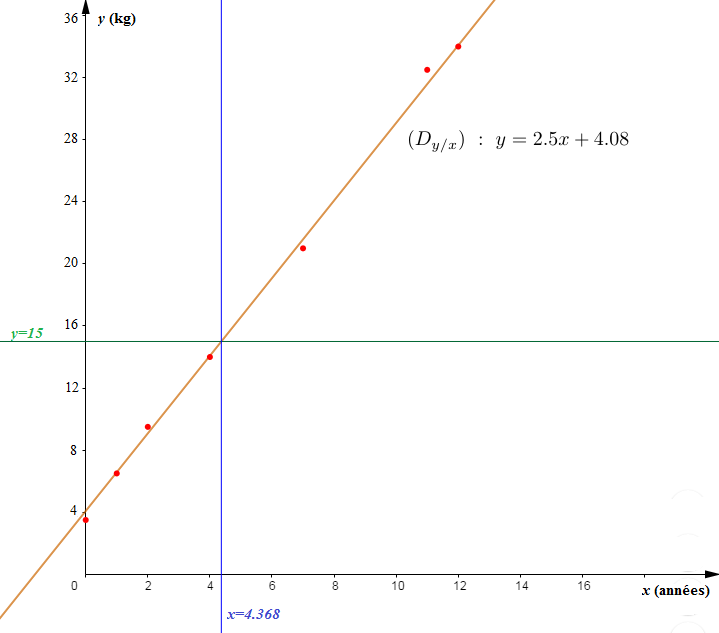
\includegraphics[width=0.8\textwidth]{CorrectionTdSta.png}
                  \label{fig:monimage}
              \end{figure}
          \end{center}
\item \( G \) a pour coordonnées \( (\bar{x},\ \bar{y}) \) avec :
\[
\bar{x} = \frac{1}{N} \sum_{i=1}^{7} x_i \simeq 5{,}28 \quad \text{et} \quad \bar{y} = \frac{1}{N} \sum_{i=1}^{7} y_i \simeq 17{,}28
\]
\item 
\begin{enumerate}
\item 
\[
\sigma_{xy} = \frac{1}{N} \sum_{i=1}^{7} x_i y_i - \bar{x} \times \bar{y} \simeq 50{,}63
\]

\[
\sigma_x = \sqrt{ \frac{1}{N} \sum_{i=1}^{7} x_i^2 - \bar{x}^2 } \simeq 4{,}66
\quad \text{et} \quad
\sigma_y = \sqrt{ \frac{1}{N} \sum_{i=1}^{7} y_i^2 - \bar{y}^2 } \simeq 11{,}39
\]

Le coefficient de corrélation linéaire est donné par la formule :
\[
r = \frac{\sigma_{xy}}{\sigma_x \times \sigma_y} \simeq 0{,}99
\]

\item \( r \) est très proche de 1, donc on a une très bonne corrélation.
\end{enumerate}
\vspace{0.5cm}

\item \( D_{y/x} \) a pour équation :
\[
y - \bar{y} = a(x - \bar{x})
\quad \text{avec} \quad a = \frac{\sigma_{xy}}{\sigma_x^2}
\]

\vspace{0.2cm}

Après calculs, on trouve qu’une équation de \( D_{y/x} \) est :
\[
y = 2{,}5x + 4{,}08
\]
\item
\begin{enumerate}
\item D’après le graphique, on constate que les valeurs de \( y \) supérieures à \( 15 \) correspondent aux valeurs de \( x \) supérieures à \( 4{,}368 \).
On ainsi dire qu’à partir de 5 ans le poids de l’enfant sera supérieur à \( 15~kg \).

\item Pour retrouver ce résultat par le calcul, on considère l’équation \( D_{y/x} \) de la droite de régression de \( y \) en \( x \).

Soit \( (D_{y/x}) : y = 2{,}5x + 4{,}08 \), alors on a :

\(
\begin{aligned}
y > 15 &\Leftrightarrow \quad 2{,}5x + 4{,}08 > 15 \\
       &\Leftrightarrow \quad 2{,}5x > 15 - 4{,}08 \\
       &\Leftrightarrow \quad x > \frac{10{,}92}{2{,}5} \\
       &\Leftrightarrow \quad x > 4{,}368
\end{aligned}
\)

D’où, \( y > 15 \ \Leftrightarrow \ x > 4{,}368 \)
\end{enumerate}
\end{enumerate}

\section*{\underline{Exercice 3}(03 points)(BAC 2009)}

\begin{enumerate}
\item \( (D_1) \) droite de régression de \( Y \) en \( X \) ayant pour équation : 
\[
y = ax + b, \text{ on a :}
\]

\[
a = \frac{\text{cov}(X, Y)}{V(X)} \qquad \text{et} \qquad b = \bar{y} - a\bar{x}
\]

\( (D_2) \) droite de régression de \( X \) en \( Y \) ayant pour équation : 
\[
x = a'y + b', \text{ on a :}
\]

\[
a' = \frac{\text{cov}(Y, X)}{V(Y)} 
\qquad \text{et} \qquad 
b' = \bar{x} - a'\bar{y}
\]

On en déduit que :

\[
\begin{aligned}
aa' &= \frac{\text{cov}(X, Y)}{V(X)} \cdot \frac{\text{cov}(Y, X)}{V(Y)} \\
    &= \frac{ \left( \text{cov}(X, Y) \right)^2 }{ V(X) \cdot V(Y) } \\
    &= \left( \frac{ \text{cov}(X, Y) }{ \sigma(X)\sigma(Y) } \right)^2 \\
    &= r^2
\end{aligned}
\]

D'où, \( \boxed{aa' = r^2} \)

\( (D_1) \) droite de régression de \( Y \) en \( X \) ayant pour équation réduite : 
\[
y = 2{,}4x, \quad \text{on a :} \quad a = 2{,}4 \quad \text{et} \quad b = 0
\]

\( (D_2) \) droite de régression de \( X \) en \( Y \) ayant pour équation réduite : 
\[
x = \frac{3{,}5}{9}y + \frac{24}{9}, \quad \text{on a :} \quad a' = \frac{3{,}5}{9} \quad \text{et} \quad b' = \frac{24}{9}
\]

D’après la question précédente, le coefficient de corrélation vérifie :
\[
\begin{aligned}
r^2 &= aa' \\
    &= 2{,}4 \times \frac{3{,}5}{9} \\
    &= \frac{14}{15}
\end{aligned}
\]

Puisque \( r = \dfrac{\text{cov}(X, Y)}{\sigma(X)\sigma(Y)} \), que \( \sigma(X) \) et \( \sigma(Y) \) sont positifs par définition et que \( \text{cov}(X, Y) \) est positif par hypothèse, alors \( r \) est positif.

Donc, \[
r = \sqrt{\dfrac{14}{15}}
\]
\item On a :
\[
\left\{
\begin{aligned}
- a\bar{x} + \bar{y} &= b \quad \text{(1)} \\
\bar{x} - a'\bar{y} &= b' \quad \text{(2)}
\end{aligned}
\right.
\]

Je garde l'équation 1. Je multiplie l'équation 2 par \( a \) pour éliminer \( \bar{x} \) :

\[
\left\{
\begin{aligned}
- a\bar{x} + \bar{y} &= b \\
a\bar{x} - aa'\bar{y} &= ab'
\end{aligned}
\right.
\]

J’additionne membre à membre : \( (1 - aa')\bar{y} = b + ab' \), c’est-à-dire :

\[
\bar{y} = \frac{b + ab'}{1 - r^2}
\]

Pour trouver \( \bar{x} \), j’utilise l’équation la plus simple ; ici c’est la 2 : \( \bar{x} = b' + a'\bar{y} \), c’est-à-dire :

\[
\begin{aligned}
\bar{x} &= b' + a'\cdot \frac{b + ab'}{1 - r^2} \\
       &= \frac{b'(1 - r^2) + a'(b + ab')}{1 - r^2} \\
       &= \frac{b' + a'b}{1 - r^2}
\end{aligned}
\]

Donc,
\[
\bar{x} = \frac{b' + a'b}{1 - r^2}
\]

Application numérique : Comme \( \dfrac{1}{1 - r^2} = 15 \), on a :

\[
\bar{y} = 15 \times 2{,}4 \times \frac{24}{9}
\qquad \text{et} \qquad
\bar{x} = 15 \times \frac{24}{9}
\]

\[
\boxed{\bar{y} = 96 \quad \text{et} \quad \bar{x} = 40}
\]

\end{enumerate}

\section*{\underline{Exercice 4}(03 points)(BAC 2010)}
On considère le tableau ci-dessous indiquant les résultats d’une étude sur le nombre d’années \( x \) en service des ouvriers d’une entreprise et de leur salaire \( y \) en milliers de francs.

\vspace{0.4cm}

Notons \( x_i \) les modalités de \( x \) et \( n_i \) l’effectif de \( x_i \), avec \( 1 \leq i \leq 6 \).

\vspace{0.2cm}

Et notons \( y_j \) les modalités de \( y \) et \( n_j \) l’effectif de \( y_j \), avec \( 1 \leq j \leq 4 \).

\vspace{0.2cm}

Soit \( N \) l’effectif total.

\vspace{0.4cm}

\[
\begin{array}{|c|c|c|c|c|c|c||c|}
\hline
x \backslash y & 2 & 6 & 10 & 14 & 18 & 22 & n_j \\
\hline
75 & a & 5 & 0 & 0 & 0 & 0 & a+5 \\
\hline
125 & 0 & 7 & 1 & 0 & 2 & 0 & 10 \\
\hline
175 & 2 & 0 & 9 & 8 & 15 & 4 & 38 \\
\hline
225 & 0 & 1 & 0 & 3 & b & 1 & b+5 \\
\hline
n_i & a+2 & 13 & 10 & 11 & b+17 & 5 & N = a + b + 58 \\
\hline
\end{array}
\]

\begin{enumerate}
    \item Déterminons \( a \) et \( b \) pour que \( \bar{x} = \dfrac{596}{59} \) et \( \bar{y} = \dfrac{8450}{59} \).

\vspace{0.3cm}

On sait que : 
\[
\bar{x} = \frac{\sum\limits_{i=1}^6 n_i x_i}{N} 
\qquad \text{et} \qquad 
\bar{y} = \frac{\sum\limits_{j=1}^4 n_j y_j}{N}
\]

\vspace{0.3cm}

Alors :
\[
\bar{x} = \frac{2(a+2) + 6 \times 13 + 10 \times 10 + 14 \times 11 + 18(b+17) + 22 \times 5}{a + b + 58}
\]

\[
\bar{y} = \frac{75(a+5) + 10 \times 125 + 38 \times 175 + 225(b+5)}{a + b + 58}
\]

\vspace{0.2cm}
Or \( \bar{x} = \dfrac{596}{59} \) et \( \bar{y} = \dfrac{8450}{59} \), d’où :

\[
\frac{2(a+2) + 6 \times 13 + 10 \times 10 + 14 \times 11 + 18(b+17) + 22 \times 5}{a + b + 58} = \frac{596}{59}
\]

\[
\frac{75(a+5) + 10 \times 125 + 38 \times 175 + 225(b+5)}{a + b + 58} = \frac{8450}{59}
\]

\vspace{0.2cm}
On obtient ainsi le système suivant :
\[
\left\{
\begin{aligned}
239a - 233b &= 4900 \\
161a - 193b &= 2580
\end{aligned}
\right.
\]

\vspace{0.2cm}
D'où \( a = 40 \quad \text{et} \quad b = 20 \)

\vspace{0.4cm}
On suppose \( a = 40 \quad \text{et} \quad b = 20 \) dans la suite.

En associant à chaque valeur \( x_i \) la moyenne \( m_i \) de la série conditionnelle \( (y/x = x_i) \), on a obtenu le tableau suivant :

\vspace{0.3cm}

\[
\begin{array}{|c|c|c|c|c|c|c|}
\hline
x & 2 & 6 & 10 & 14 & 18 & 22 \\
\hline
m & 80 & 113 & 170 & 189 & 199 & 185 \\
\hline
\end{array}
\]
\item 
\begin{enumerate}
  \item Calculons le coefficient de corrélation linéaire.
    \item Déterminons d'abord les moyennes \( \bar{x} \) et \( \bar{m} \), les variances \( V_x \), \( V_m \), les écarts-types \( \sigma_x \), \( \sigma_m \), et la covariance de \( x \) et \( m \).

    Notons que la série statistique double \( (x, m) \) est injective.

    \[
    \bar{x} = \frac{1}{N} \sum\limits_{i=1}^{6} x_i 
    \qquad , \qquad 
    \bar{m} = \frac{1}{N} \sum\limits_{i=1}^{6} m_i
    \]

    \[
    V_x = \frac{1}{N} \sum\limits_{i=1}^{6} x_i^2 - \bar{x}^2 
    \qquad , \qquad 
    V_m = \frac{1}{N} \sum\limits_{i=1}^{6} m_i^2 - \bar{m}^2
    \]

    \[
    \sigma_x = \sqrt{V_x}, \qquad 
    \sigma_m = \sqrt{V_m}, \qquad 
    \text{et} \quad \text{cov}(x, m) = \frac{1}{N} \sum\limits_{i=1}^{6} x_i m_i - \bar{x}\bar{m}
    \]

    \[
    \bar{x} = 12, \quad 
    \bar{m} = 156, \quad 
    V_x \simeq 46{,}66, \quad 
    V_m \simeq 1933{,}33
    \]

    \[
    \sigma_x \simeq 6{,}83, \quad 
    \sigma_m \simeq 43{,}96, \quad 
    \text{cov}(x, m) \simeq 267{,}33
    \]
    
    \item Calculons maintenant le coefficient de corrélation linéaire \( r \) :

    \[
    r = \frac{\text{cov}(x, m)}{\sigma_x \sigma_m}
    \]

    D'où \( r \simeq 0{,}89 \)

    Puisque \( r \) est proche de 1, il y a alors une forte corrélation entre \( x \) et \( m \).
    \item La droite de régression de \( m \) en \( x \), notée \( D_{m/x} \), a pour équation \( m = ax + b \) avec :

  \[
  a = \frac{\text{cov}(x, m)}{V_x} 
  \qquad \text{et} \qquad 
  b = \bar{m} - a \bar{x}
  \]

  \[
  \Rightarrow \quad D_{m/x} : \quad m = 5{,}73x + 87{,}25
  \]

   \item Si \( x = 30 \), alors \( m \simeq 259{,}128 \). D'où le salaire moyen d'un ouvrier ayant 30 ans d'ancienneté est sensiblement égal à \textbf{259130 F}.

  \end{enumerate}
\end{enumerate}
\section*{\underline{Exercice 5}(05 points)(BAC 2013)}
\begin{enumerate}
    \item 
    \begin{enumerate}
        \item Soit : 
        \[
        r = \frac{\text{cov}(X, Y)}{\sigma_X \sigma_Y}
        \]
        Donc, \( r = -0{,}973 \)

        Ce qui signifie qu'il y a une forte corrélation.

        \item[b)] La droite de régression de \( Y \) en \( X \) est :
        \[
        y = ax + b \quad \text{avec} \quad 
        a = \frac{\text{cov}(X, Y)}{V(X)} 
        \quad \text{et} \quad 
        b = \bar{Y} - a\bar{X}
        \]
        \[
        \Rightarrow \quad y = -0{,}874x + 4{,}12
        \]

        Ainsi, 
        \fbox{\( y = -0{,}874x + 4{,}12 \)}

        \item Si \( x = 6 \) alors \( y \simeq -1{,}124 \)

        Cette équation ne permet pas d'estimer le degré de salinité car au \( 6^{\text{ième}} \) mois de pluie, le degré de salinité ne peut être négatif.
    \end{enumerate}

    \item \( Z = \ln(Y - 1) \)

    \begin{enumerate}
        \item Le tableau correspondant à la série \( (X, Z) \) est donné par :

        \[
        \begin{array}{|c|c|c|c|c|c|c|}
        \hline
        X_i & 0 & 1 & 2 & 3 & 4 \\
        \hline
        Z_i & 1{,}182 & 0{,}875 & 0{,}010 & -1{,}830 & -4{,}610 \\
        \hline
        \end{array}
        \]

    \item  Le coefficient de corrélation linéaire de cette série \( (X, Z) \) est :
        \[
        r = \frac{\text{cov}(X, Z)}{\sigma_X \sigma_Z} = -0{,}944
        \]

        La droite de régression de \( Z \) en \( X \) est :
        \[
        z = ax + b \quad \text{avec} \quad a = \frac{\text{cov}(X, Z)}{V(X)} 
        \quad \text{et} \quad 
        b = \bar{Z} - a\bar{X}
        \]
        \[
        \Rightarrow z = -1{,}428x + 1{,}982
        \]
        D'où, 
        \fbox{\( z = -1{,}428x + 1{,}982 \)}

        \item Exprimons \( Y \) en fonction de \( X \).
        \( \text{On a : } z = \ln(y - 1) \quad \text{et} \quad z = -1{,}428x + 1{,}982 \text{ d'où,}\)
\(
\begin{aligned}
\ln(y - 1) = -1{,}428x + 1{,}982 &\quad \Rightarrow \quad y - 1 = e^{-1{,}428x + 1{,}982} \\
                                 &\quad \Rightarrow \quad y = e^{-1{,}428x + 1{,}982} + 1
\end{aligned}
\)

Ainsi, \fbox{\( y = e^{-1{,}428x + 1{,}982} + 1 \)}
    \item Si \( x = 6 \) alors, \( y = 1{,}001 \). Le degré de salinité estimé au \( 6^{\text{ième}} \) mois est positif, il est très proche de celui du quatrième mois et lui est inférieur.
    
    Donc, l'équation \( y = e^{-1{,}428x + 1{,}982} + 1 \) nous permet de faire cette estimation.

    \end{enumerate}
\end{enumerate}
\section*{\underline{Exercice 6}(02,5 points)(BAC 2015)}
\begin{enumerate}
    \item Le coefficient de corrélation linéaire \( r \) est défini par 
    \[
    r = \frac{\text{Cov}(X, Y)}{\sigma_X \sigma_Y}.
    \]
    D'où : \( r \approx \mathbf{0{,}69} \).

    \item 
    \begin{enumerate}

            \item La droite de régression de \( Y \) en \( X \), \( (D_{Y/X}) \), a pour équation \( y = \mathbf{92{,}59x - 4{,}35} \).

            \item Il faut investir \( 3{,}29 \) milliards de \( \mathit{FCFA} \) si l'on désire un chiffre d'affaire de 300 milliards.

    \end{enumerate}
\end{enumerate}
\end{document}
